\section{Experimental Results}
% [WRITING GUIDANCE]
% Target length: 1.5 - 2 columns.
% Present the quantitative results of the models.

\subsection{Hyperparameter Optimization}
% Discuss how GridSearchCV was used, specifically for k-NN (k=3,5,7,9,11) on the training set.

% Insert Hyperparameter Comparison Table
\begin{table}[htbp]
\caption{Hyperparameter Optimization Results (e.g., k-NN)}
\begin{center}
\begin{tabular}{|c|c|}
\hline
\textbf{Hyperparameter ($k$)} & \textbf{CV F1-Score} \\
\hline
3 & 0.xx \\
5 & 0.xx \\
7 & 0.xx \\
\hline
\end{tabular}
\label{tab:hyperparams}
\end{center}
\end{table}

\subsection{Model Comparison}
% Compare the final performance of all classifiers on the test set.

% Insert Final Evaluation Metrics Table
\begin{table}[htbp]
\caption{Final Evaluation Metrics on Test Set}
\begin{center}
\begin{tabular}{|l|c|c|c|c|}
\hline
\textbf{Model} & \textbf{Precision} & \textbf{Recall} & \textbf{F1-Score} & \textbf{ROC-AUC} \\
\hline
Decision Tree & 0.xx & 0.xx & 0.xx & 0.xx \\
Naive Bayes & 0.xx & 0.xx & 0.xx & 0.xx \\
k-NN & 0.xx & 0.xx & 0.xx & 0.xx \\
Random Forest & 0.xx & 0.xx & 0.xx & 0.xx \\
\hline
\end{tabular}
\label{tab:final_metrics}
\end{center}
\end{table}

% Insert Figure 4 here. (ROC Curves)
\begin{figure}[htbp]
\centerline{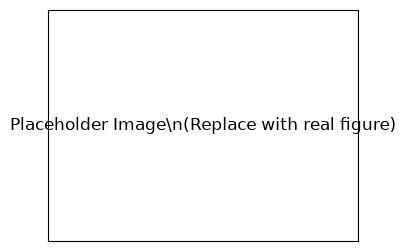
\includegraphics[width=\columnwidth]{figures/placeholder.png}}
\caption{ROC Curves for compared classifiers.}
\label{fig:roc}
\end{figure}

% Insert Figure 5 here. (Precision-Recall Curves)
\begin{figure}[htbp]
\centerline{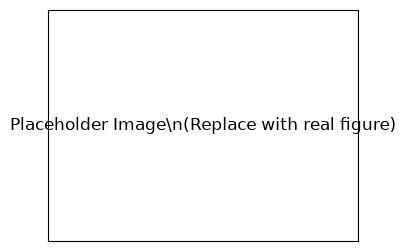
\includegraphics[width=\columnwidth]{figures/placeholder.png}}
\caption{Precision-Recall Curves for compared classifiers.}
\label{fig:pr}
\end{figure}

% Insert Figure 8 here. (Confusion Matrix)
\begin{figure}[htbp]
\centerline{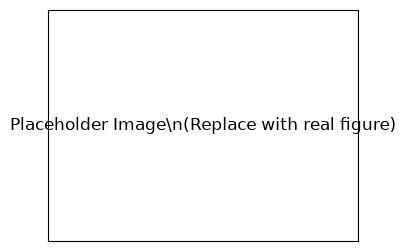
\includegraphics[width=0.8\columnwidth]{figures/placeholder.png}}
\caption{Confusion Matrix for the best performing model.}
\label{fig:conf_matrix}
\end{figure}

% Discuss why Random Forest (or the best model) outperformed Decision Tree or Naive Bayes.
% Write your results description here...
